\documentclass{beamer}
\usepackage[polish]{babel}
\usepackage[utf8]{inputenc}

\usepackage{movie15}
\usepackage{hyperref}
\usepackage{wrapfig}


\usepackage{caption}


%\usepackage{algorithm2e}
%\usepackage{algorithmic}
%\usepackage{float}
%\usepackage[noend]{algpseudocode}

\usepackage{algorithmic}

\usepackage[absolute,overlay]{textpos}
\usepackage{graphicx}

%https://gist.github.com/andrejbauer/ac361549ac2186be0cdb
\usepackage{pgfpages}
\usetheme{AGH}

%\setbeameroption{hide notes} % Only slides
%\setbeameroption{show only notes} % Only notes
\setbeameroption{show notes on second screen=right} % Both


% Give a slight yellow tint to the notes page
\setbeamertemplate{note page}{\pagecolor{yellow!5}\insertnote}\usepackage{palatino}

\title{Behawioralny algorytm koordynacji ruchu robotów mobilnych oparty na modelu postępowania przemieszczających się osób}
\author{Szymon Szomiński}
%\institute{Katedra Telekomunikacji}
%\website{\url{http://www.kt.agh.edu.pl/~wydrych/}}
\date{\today}

\begin{document}
	
\titleframe[pl]
	
\begin{frame}
	\frametitle{Agenda}
	\tableofcontents
\end{frame}

\section{Inspiracja -- zjawisko respektu}
\begin{frame}
\frametitle{\secname}

Wkleić zdjęcia oraz tekst

\end{frame}

\section{Zjawisko respektu}
\begin{frame}
\frametitle{\secname}

\begin{textblock*}{5cm}(0.3\linewidth,2cm) % {block width} (coords)
	\begin{equation*}
	k_j = \sum_{i \in Z}  \left(   \frac{D_{max} - d_{ij}}{D_{max}} ~ \cdot ~ cos(\phi_{ij}) ~ \cdot f_i \right)
	\end{equation*}
\end{textblock*}

\begin{textblock*}{5cm}(7cm,4.2cm) % {block width} (coords)
	\scriptsize{
		\begin{tabular}{lp{0.85\textwidth}}
			$ k_j $       	& Współczynnik respektu dla \textit{j--tego} robota. \\
			$ d_{ij} $    	& Odległość pomiędzy robotem \textit{i--tym} oraz \textit{j-tym}. \\
			$ \phi_{ij} $ 	& Kąt skierowany pomiędzy robotem \textit{i--tym} oraz \textit{j--tym}. \\
			$ f_i $ 		& Bazowy współczynnik respektu dla \textit{i-tego} robota. Znany wszystkim uczestnikom ruchu oraz stały w czasie wyznaczania trajektorii ruchu przez wszystkich robotów. \\
			$ D_{max} $ 	& Zasięg.  \\
			$ Z $ 			& Zbiór robotów znajdujących się w zasięgu $ D_{max} $ \textit{j-tego} robota.	
	\end{tabular}}
\end{textblock*}

\begin{textblock*}{6cm}(1cm,5cm) % {block width} (coords)
	\includegraphics[page=5,width=6cm]{img/hybrid_algorithm.pdf}
\end{textblock*}

\note{Wprowadzono sztuczną funkcję używaną do określenia, który robot posiada większy stopień respektu. Roboty nie negocjują ani nie wymieniają się żadnymi informacjami potrzebnymi do wyliczenia współczynnika. Żadnemu z robotów nie przypisuje się również odgórnie konkretnego stopnia respektu. Każdy z robotów autonomicznie, w sposób całkowicie zdecentralizowany wylicza wartość \textit{współczynnika respektu}, bazując wyłączenie na obserwacji innych uczestników ruchu. \textit{Współczynnik respektu} reprezentowany jest przez pojedynczą wartość zmiennoprzecinkową $ k_j $ obliczaną według wzoru:}

\note{W przestrzeni w której nie wystębuje duża ilość przeszkud statycznych oraz roboty moga sfobodnie się przemiszczać zjawiko raspketu może być z powodzeniem stosowane. Stworzono dwa algorytmu bazające na Zjawisku Respektu: R oraz R+}

\note{Bazując na \textit{zjawisku respektu} stworzono dwie metody, których działania wykorzystują jego właściwości.}

\end{frame}	

\subsection{Pseudo-kod implementacja algorytmu Respect (R)}
\begin{frame}
\frametitle{\subsecname}
\scriptsize{		
	\begin{algorithmic}[1]	
		\REPEAT
		
		\STATE $ goal_{i} = \Upsilon(pos_{i}) $
		
		\STATE $ Z \gets RobotsWithFixedDistance(pos_{i},Rob) $
		\STATE $ k_{i} \gets k(pos_{i},Z) $
		
		\STATE  $ robotsWithLowerRespectTooClose \gets GetLowerRespectRobots(k_{i},Z) $
		
		\STATE  $ robotsWithHigherRespect \gets GetHigherRespectRobots(k_{i},Z) $
		
		\IF{$ robotsWithLowerRespectTooClose.Count > 0 $}
		\STATE	$ \kappa(i, robotsWithLowerRespectTooClose) $ 
		\ELSE			
		\IF{$ robotsWithHigherRespect.Count > 0 $}
		\STATE $ \kappa(i, robotsWithHigherRespect) $
		\ELSE	
		\STATE $ \kappa(i, r_{i}) $ 
		\ENDIF
		\ENDIF
		\UNTIL{$ goal_{i} \neq \varnothing $}	
\end{algorithmic}}

\note{Pierwszy z algorytmów został nazwany Respect (R). Listing  przedstawia implementację w pseudo-kodzie poszczególnych kroków działania algorytmu R.}

\note{Algorytm \textit{R} pobiera lokalizacje uczestników ruchu (linia: 4), wyznacza swój \textit{współczynnik respektu} zgodnie ze wzorem \ref{eq:fearFactor} (linia: 5). W kolejnym etapie metoda sprawdza czy trajektoria robota koliduje z trajektoriami pozostałych uczestników ruchu, czy też nie (linie: 6-7). Jeżeli trasa pokrywa się z trasą innego robota, w celu wyznaczenia pierwszeństwa dokonywane jest porównanie obliczonych \textit{współczynników respektu}. Gdy \textit{współczynnik respektu} jest mniejszy  niż \textit{współczynnik respektu} robota kolidującego, robot zmuszony jest do ustąpienia mu pierwszeństwa i wyznaczenia nowej trasy (linia: 12). Jeżeli trajektoria robota nie koliduje z robotem o większym \textit{współczynniku respektu}, robot wyznacza najkrótsza trasę do celu wykorzystując algorytm \cite{TurekCetnarowiczZaborowski2011} (linia: 14). Do wyznaczenia nowej bezkolizyjnej ścieżki w~algorytmie \textit{R} brane są pod uwagę wyłącznie te roboty, których obliczone \textit{współczynniki respektu} są większe od \textit{współczynnika respektu} bieżącego robota (linia: 12). Algorytm zakłada, iż roboty o mniejszym \textit{współczynniku respektu} ustąpią pierwszeństwa robotowi o wyższym \textit{współczynniku respektu}. Procedura powtarzana jest dopóty, dopóki wszystkie cele robota nie zostaną osiągnięte (linia: 15).}
\end{frame}

\subsection{Pseudo-kod implementacja algorytmu Respect+ (R+)}
\begin{frame}
\frametitle{\subsecname}
\scriptsize{		
\begin{algorithmic}[1]	
	
	\REPEAT
	
	\STATE $ goal_{i} = \Upsilon(pos_{i}) $
	
	\STATE $ Z \gets RobotsWithFixedDistance(pos_{i},Rob) $
	\STATE $ k_{i} \gets k(pos_{i},Z) $
	
	\STATE  $ robotsWithLowerRespectTooClose \gets GetLowerRespectRobots(k_{i},Z) $
	
	\STATE  $ robotsWithHigherRespect \gets GetHigherRespectRobots(k_{i},Z) $
	
	\STATE  $ allCollisionRobots \gets GetAllCollisionRobots(k_{i},Z) $
	
	\IF{$ robotsWithLowerRespectTooClose.Count > 0 $}
	\STATE	$ \kappa(i, robotsWithLowerRespectTooClose) $ 
	\ELSE			
	\IF{$ robotsWithHigherRespect.Count > 0 $}
	\STATE $ \kappa(i, robotsWithHigherRespect) $
	\ELSE	
	\STATE $ \kappa(i, allCollisionRobots) $ 
	\ENDIF
	\ENDIF
	\UNTIL{$ goal_{i} \neq \varnothing $}
\end{algorithmic}}

\note{Listing przedstawia implementację w pseudo-kodzie poszczególnych kroków działania algorytmu Respect+ (R+)}

\note{Metoda Respect+ (R+), podobnie jak metoda Respect (R), pobiera lokalizacje robotów (linia: 4), oblicza \textit{współczynnik respektu} (linia: 5), lecz wyznaczanie trajektorii ruchu przebiega w nieco odmienny sposób. W algorytmie \textit{R+} robot, który nie musi ustąpić pierwszeństwa ruchu przejazdu innym robotom, stara się pokonać trasę do celu bez modyfikowania swojej trajektorii. Jeżeli jednak nie jest możliwy bezkolizyjny ruch, dokonywana jest korekcja trajektorii uwzględniająca bieżącą pozycję innych uczestników ruchu (linia: 15). Robot, którego obliczony współczynnik respektu jest mniejszy od współczynników respektu pozostałych uczestników ruchu, zobligowany jest do zmiany swojej trasy w celu ustąpienia pierwszeństwa (linia: 13).}

\end{frame}

\section{Zasada priorytetyzowania wychodzących}
\begin{frame}
\frametitle{\secname}

\begin{textblock*}{5cm}(0.3\linewidth,1.5cm) % {block width} (coords)
	\begin{equation*}
	p_j = 1 + \psi\left(d_{jl}\right) * \lambda\left(\alpha_j,\gamma_l\right) * \tau 
	\end{equation*}
\end{textblock*}

\begin{textblock*}{5cm}(0.1\linewidth,2.5cm) % {block width} (coords)
	\footnotesize{
		\begin{equation*}
		\psi\left(d_{jl}\right) = \left\{\begin{array}{ll}
		\frac{R_{l} - d_{jl}}{R_{l}} \mbox{ dla } d_{jl} \le R_{l} \\
		0 \mbox{ w innym przypadku }        
		\cr
		\end{array}\right.
		\end{equation*}
	}
\end{textblock*}

\begin{textblock*}{5cm}(0.6\linewidth,2.5cm) % {block width} (coords)
	\footnotesize{
		\begin{equation*}
		\lambda\left(\alpha_j,\gamma_l\right) = \left\{\begin{array}{ll}
		1  \mbox{ dla } - \frac{\pi}{2} \leq \alpha_j - \gamma_l \leq \frac{\pi}{2} \\
		0  \mbox{ w innym przypadku }
		\cr
		\end{array}\right.
		\end{equation*}	
	}
\end{textblock*}

\begin{textblock*}{4.8cm}(7cm,3.8cm) % {block width} (coords)
	\scriptsize{
		\begin{tabular}{lp{0.85\textwidth}}
			$ p_j $ 						& Czynnik przejścia przez drzwi dla  \textit{j-tego} robota.\\
			$ \psi\left(d_{jl}\right) $ 	& Funkcja określająca w jakim stopniu robot jest w zasięgu działania drzwi.\\
			$ \lambda(\alpha_j,\gamma_l) $ 	& Funkcja, która decyduje czy robot \textit{j-ty} wchodzi do pomieszczenia, czy wychodzi z niego.\\
			$ \tau \in \mathbb{R}_{+} $ 	& Współczynnik definiujący wpływ czynnika przejścia na pierwszeństwo.\\
			$ d_{jl} $ 						& Dystans pomiędzy robotem \textit{j-tym} oraz środkiem \textit{l-tego} przejścia.\\
			$ l $ 							& Identyfikator przejścia (drzwi). \\
			$ \gamma_l $ 					& Kąt skierowania wersora wskazującego kierunek ,,wychodzenia'' przez drzwi.
		\end{tabular}
	}
\end{textblock*}

\begin{textblock*}{6cm}(1cm,5cm) % {block width} (coords)
	\includegraphics[page=6,width=6cm]{img/hybrid_algorithm.pdf}
\end{textblock*}

%\note{Gdzie:
%	pj       - Czynnik przejścia przez drzwi dla robota  j .
%	ψ(djl)  - Funkcja określająca, w jakim stopniu robot jest w zasięgu działania drzwi.
%	λ(αj,γl) - Funkcja która decyduje, czy robot j wchodzi do pomieszczenia czy wychodzi z niego.
%	τ ϵ R+    - Współczynnik definiujący wpływ czynnika przejścia na pierwszeństwo. W eksperymentach przyjęliśmy wartość  τ = 1, ale możliwe jest dynamiczne określanie tego współczynnika na przykład na podstawie stosunku zagęszczeń robotów w sąsiadujących pomieszczeniach.
%	djl  - Dystans pomiędzy robotem  j  oraz środkiem przejścia (drzwiami)  l  (można zmienić na odległość od odcinka stanowiącego drzwi).
%	l - Identyfikator drzwi. Lokalizacja drzwi, ich szerokość oraz kierunek otwarcia zdefiniowane zostały w pliku mapy labiryntu i są dostępne dla każdego z robotów.
%	γl  - kąt prostopadły do odcinka reprezentującego drzwi, wskazujący kierunek ,,wychodzenia'' przez drzwi. 
%	Rl  - Maksymalny zasięg działania drzwi l.}

\end{frame}

\section{Integracja zjawiska respektu z czynnikiem przejścia przez drzwi}
\begin{frame}
\frametitle{\secname}

\begin{textblock*}{5cm}(0.4\linewidth,2cm) % {block width} (coords)
	\begin{equation*}
	KP_j = k_j * p_j
	\end{equation*}
\end{textblock*}

\begin{textblock*}{6cm}(0.25\linewidth,3cm) % {block width} (coords)
	\includegraphics[page=1,width=8cm]{img/AlgorytmPrzejsciaPrzezDrzwi.pdf}
\end{textblock*}

\note{W oparciu o rozrzeszoną metodę Passage Factor (PF) oraz jego odmianę PF+. Algorytm PF wykorzystuje właściwości algorytmu \textit{R} uzupełnionego o zasadę priorytetyzowania robotów w trakcie opuszczania pomieszczenia.}

\end{frame}

\subsection{Pseudo-kod implementacja algorytmu Passage Factor (PF)}
\begin{frame}
\frametitle{\subsecname}
\scriptsize{		
	\begin{algorithmic}[1]
		
		\REPEAT
		
		\STATE $ goal_{i} = \Upsilon(pos_{i}) $
		
		\STATE $ Z \gets RobotsWithFixedDistance(pos_{i},Rob) $
		\STATE $ door_{l} \gets GetDoorFromMap(l) $
		\STATE $ kp_{i} \gets KP(pos_{i}, Z, door_{l}) $
		
		\STATE  $ robotsWithLowerRespectTooClose \gets GetLowerRespectRobots(kp_{i},Z) $
		
		\STATE  $ robotsWithHigherRespect \gets GetHigherRespectRobots(kp_{i},Z) $
		
		\IF{$ robotsWithLowerRespectTooClose.Count > 0 $}
		\STATE	$ \kappa(i, robotsWithLowerRespectTooClose) $ 
		\ELSE			
		\IF{$ robotsWithHigherRespect.Count > 0 $}
		\STATE $ \kappa(i, robotsWithHigherRespect) $
		\ELSE	
		\STATE $ \kappa(i, r_{i}) $ 
		\ENDIF
		\ENDIF
		\UNTIL{$ goal_{i} \neq \varnothing $}
		
\end{algorithmic}}
\end{frame}		


\subsection{Pseudo-kod implementacja algorytmu  Passage Factor (PF+)}
\begin{frame}
\frametitle{\subsecname}
\scriptsize{		
\begin{algorithmic}[1]
	\REPEAT
	
	\STATE $ goal_{i} = \Upsilon(pos_{i}) $
	
	\STATE $ Z \gets RobotsWithFixedDistance(pos_{i},Rob) $
	
	\STATE $ door_{l} \gets GetDoorFromMap(l) $
	\STATE $ kp_{i} \gets KP(pos_{i}, Z, door_{l}) $
	
	\STATE  $ robotsWithLowerRespectTooClose \gets GetLowerRespectRobots(kp_{i},Z) $
	
	\STATE  $ robotsWithHigherRespect \gets GetHigherRespectRobots(kp_{i},Z) $
	
	\STATE  $ allCollisionRobots \gets GetAllCollisionRobots(kp_{i},Z) $
	
	\IF{$ robotsWithLowerRespectTooClose.Count > 0 $}
	\STATE	$ \kappa(i, robotsWithLowerRespectTooClose) $ 
	\ELSE			
	\IF{$ robotsWithHigherRespect.Count > 0 $}
	\STATE $ \kappa(i, robotsWithHigherRespect) $
	\ELSE	
	\STATE $ \kappa(i, allCollisionRobots) $ 
	\ENDIF
	\ENDIF
	\UNTIL{$ goal_{i} \neq \varnothing $}	
	
\end{algorithmic}}
\end{frame}		

\section{Zasada prawej dłoni}
\begin{frame}
\frametitle{\secname}
\framesubtitle{Pseudo-kod implementacja algorytmu  Priority to the Right (PR)}
\scriptsize{		
	\begin{algorithmic}[1]
		
		\REPEAT
		
		\STATE $ goal_{i} = \Upsilon(pos_{i}) $
		
		\STATE $ Z \gets RobotsWithFixedDistance(pos_{i},Rob) $
		
		\STATE $ robotsOnTheRightSide \gets GetRobotOnTheRightSide(pos_{i}) $
		
		\IF{$ robotsOnTheRightSide.Count > 0 $}
		\STATE	$ \kappa(i, robotsOnTheRightSide) $ 
		\ELSE			
		\STATE $ \kappa(i, r_{i}) $ 
		\ENDIF
		
		\UNTIL{$ goal_{i} \neq \varnothing $}
		
\end{algorithmic}}

\note{Inspiracją do za-modelowania \textit{zasada prawej dłoni} została zapożyczona z prawa ruchu drogowego oraz reguł poruszania się obowiązujących na wodzie. W środowisku, w~którym poruszają się roboty rzadko spotyka się wyznaczone pasy ruchu.
	
W stworzonej metodzie pierwszeństwo poruszania się mają roboty nadjeżdżające z~prawej strony. Na listingu zaprezentowano kolejne etapy działania algorytmu PR.}

\note{Jeżeli robot wykryje robota nadjeżdżającego z prawej strony, to w zaistniałej sytuacji zobligowany jest do ustąpienia mu pierwszeństwa. Robot zmienia swoją dotychczasową trajektorię ruchu starając się ominąć robota zbliżającego się z prawej strony (linia: 7). Gdy roboty wzajemnie się wyminą, robot wyznacza trajektorię do celu (linia: 9), aby powrócić do wykonywania powierzonego zadania.}

\end{frame}		

\section{Eksperyment na rzeczywistych robotach}
\begin{frame}
\frametitle{\secname}

\begin{itemize}
	\item Obudowa A4WD1v2 Lynxmotion 22cm x 20cm x 6cm.
	\item Zasilanie dwie baterie litowo-polimerowe o nominalnym napięciu 14.8V i pojemności 5Ah.
	\item Sterowniki silników RoboClaw 2 x 15A firmy BasicMicro.
	\item Komputer sterujący PandaBoard ES:	
	\begin{itemize}
		\item dwurdzeniowy procesor Cortex-A9 OMAP4460 taktowany zegarem 1,2 GHz,
		\item RAM 1GB,
		\item Ethernet RJ45 100Mb,
		\item WiFi 802.11 b/g/n i Bluetooth 2.1,
		\item USB 2.0,
		\item I2C,
		\item SPI.
	\end{itemize}
	\item Skaner laserowy URG-04LX-UG01 firmy Hokuyo.	
\end{itemize}

\begin{textblock*}{4cm}(8.5cm,5.2cm) % {block width} (coords)
	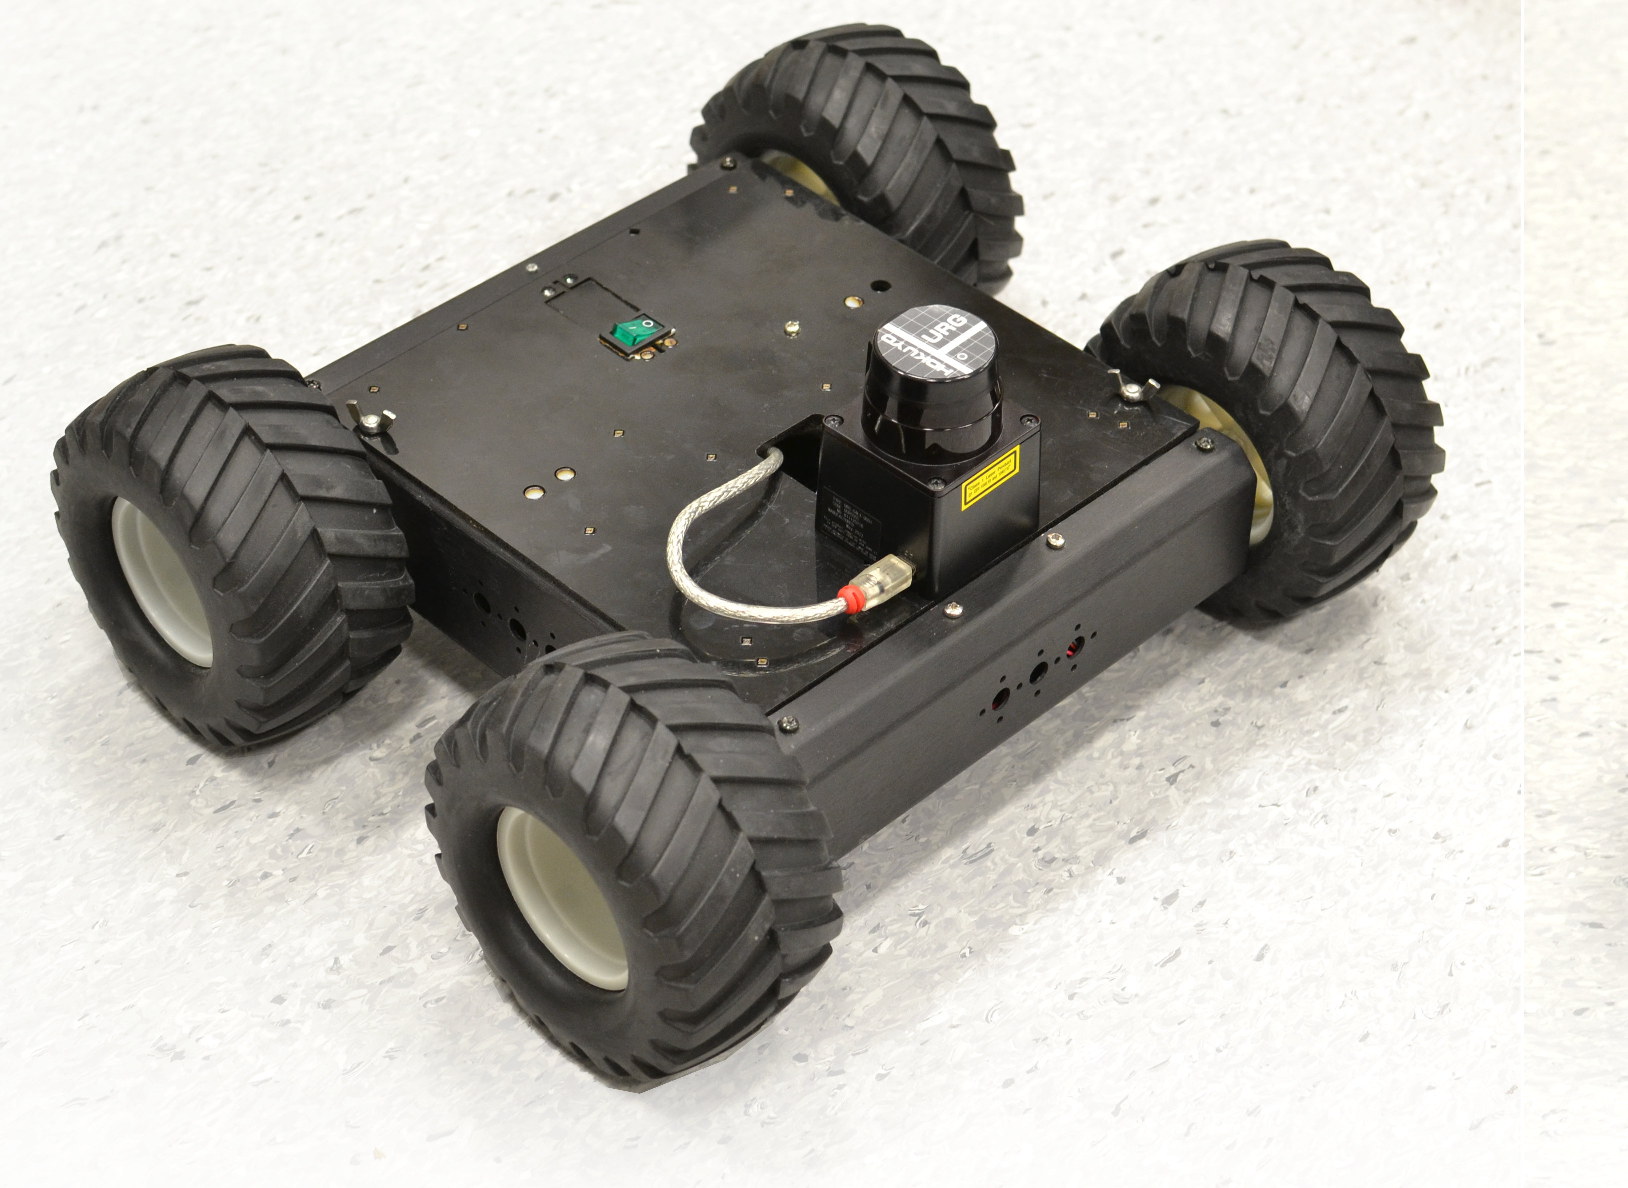
\includegraphics[page=1,width=4cm]{img/Rysunki.pdf}
\end{textblock*}

\tiny{
Open Source Hardware \\
Strona projektu: \url{http://capo.iisg.agh.edu.pl/}}

\note{W celu zweryfikowania poprawności działania algorytmów wykorzystano platformę CAPO }
\end{frame}





















	



\end{document}






%
%
%
%
%
%
%\documentclass[notes]{beamer}       % print frame + notes
%%\documentclass[notes=only]{beamer}   % only notes
%%\documentclass{beamer}              % only frames
%
%
%%\setbeameroption{show notes on second screen=right} % Both
%
%% Give a slight yellow tint to the notes page
%\setbeamertemplate{note page}{\pagecolor{yellow!5}\insertnote}\usepackage{palatino}
%
%\usepackage[polish]{babel}
%\usepackage[utf8]{inputenc}
%\usepackage{lmodern}
%
%\usetheme{AGH}
%

%
%\begin{document}
%
%\titleframe[pl]
%
%\begin{frame}
%\frametitle{Zwykły slajd...}
%\framesubtitle{...z podtytułem...}
%    \begin{itemize}[<+-|alert@+>]
%        \item ...i zwykłą treścią.
%    \end{itemize}
%\note{Everything you want}
%\end{frame}
%
%
%
%\begin{frame}
%\frametitle{Inspiracja – zjawisko respektu}
%
%\begin{itemize}[<+-|alert@+>]
%	\item ...i zwykłą treścią.	
%\end{itemize}
%\end{frame}

%
%\section{Zwykły slajd... ala ma kota szsz}	
%\begin{frame}
%\frametitle{\secname}
%%\framesubtitle{...z podtytułem...}
%
%\begin{itemize}
%	\item Here are
%	\item some very boring bullets
%	\item about nothing.
%\end{itemize}
%
%\note[item]{Note that this slide is boring.}
%
%\note[item]{Observe that there are no actual bullets here.}
%
%\note[item]{Future work: add another bullet.}
%\end{frame}
%
%
%\section{Zwykły 2}	
%\begin{frame}
%\frametitle{\secname}
%%\framesubtitle{...z podtytułem...}
%
%\begin{itemize}
%\item Here are
%\item some very boring bullets
%\item about nothing.
%\end{itemize}
%
%\note[item]{Note that this slide is boring. 1233}
%\end{frame}
%
%\section{teee}
%\begin{frame}
%\frametitle{\secname}
%%\framesubtitle{...z podtytułem...}
%
%Jakis długi teskt a pod nim filmiki:fdgfdsfgdsfds fds 
%fdsf
%dsfdsf
%dsf
%dsf
%ds dfd
%
%Jakis  ubtt tejst
%
%\begin{itemize}
%\item znam robota
%\item nie wiem gdzie jest
%\end{itemize}
%
%
%\begin{figure}[!hb]
%
%\includemovie[autoplay,repeat]{3cm}{3cm}{mov/test2.mpg}
%\includemovie[autoplay,repeat]{3cm}{3cm}{mov/test3.mpg}
%\includemovie[autoplay,repeat]{3cm}{3cm}{mov/test4.mpg}
%\end{figure}
%
%\end{frame}

%
%
%\end{document}
